\documentclass[12pt, letterpaper]{article}
\date{\today}
\usepackage[margin=1in]{geometry}
\usepackage{amsmath}
\usepackage{cancel}
\usepackage{amssymb}
\usepackage{fancyhdr}
\usepackage{pgfplots}
\usepackage{booktabs}
\usepackage{pifont}
\usepackage{amsthm,latexsym,amsfonts,graphicx,epsfig,comment}
\pgfplotsset{compat=1.16}
\usepackage{xcolor}
\usepackage{tikz}
\usetikzlibrary{shapes.geometric}
\usetikzlibrary{arrows.meta,arrows}
\usepackage{pdfpages}
\usepackage{hyperref}


\newcommand{\Z}{\mathbb{Z}}
\newcommand{\N}{\mathbb{N}}
\newcommand{\R}{\mathbb{R}}
\newcommand{\Q}{\mathbb{Q}}
\newcommand{\C}{\mathbb{C}}
\newcommand{\F}{\mathbb{F}}

\newcommand{\Po}{\mathcal{P}}
\newcommand{\Pro}{\mathbb{P}}
\author{Alex Valentino}
\title{Numerical Analysis homework}
\pagestyle{fancy}
\renewcommand{\headrulewidth}{0pt}
\renewcommand{\footrulewidth}{0pt}
\fancyhf{}
\rhead{
	Homework 3\\
	Numerical Analysis
}
\lhead{
	Alex Valentino\\
	Collaborators: Irshad Guliyev (iag38), Jay Patwardhan (jap600)
}
\begin{document}
	\begin{itemize}
		\item{Question 1}\textit{
			Consider a polynomial of degree 3:
			$$
			p(x) = a_0 + a_1 x + a_2 x^2 + a_3 x^3
			$$		
		where $a_0,a_1,a_2,a_3$ are unknown coeffcients.  We know that $y = p(x)$ passes through 4 distinct points
		$(x_1,y_1),(x_2,y_2),(x_3,y_3),(x_4,y_4),$ that is, 
		$$
		y_i = p(x_i), \text{ for } i = 1,2,3,4
		$$
		Convert the problem of finding the coefficents in $p(x)$ into solving a system of linear equations
		}\\
		Solving for $a_0, a_1, a_2, a_3$ as a matrix equation can be done in the following way:  
		$$
		\begin{bmatrix}
		1 & x_1 & x_1^2 & x_1^3\\
		1 & x_2 & x_2^2 & x_2^3\\
		1 & x_3 & x_3^2 & x_3^3\\
		1 & x_4 & x_4^2 & x_4^3
		\end{bmatrix}
		\begin{bmatrix}
	 	a_0\\ a_1\\ a_2\\ a_3
	 	\end{bmatrix}
	 	= 
	 	\begin{bmatrix}
		y_1\\ y_2\\ y_3\\ y_4
		\end{bmatrix}
		$$
		Note we can do this via observing that 
		\begin{align*}
			y_i &= p(x_i)\\
			&= a_0 + a_1 x_i + a_2 x_i^2 + a_3 x_i^3\\
			&= \begin{bmatrix}
			1 & x_i & x_i^2 & x_i^3
			\end{bmatrix}
			\begin{bmatrix}
	 	a_0\\ a_1\\ a_2\\ a_3
	 	\end{bmatrix}
		\end{align*}
		Therefore we have four independent equations, thus they can be solved as a system of linear equations in the 
		matrix form as shown above.  
		\item{Question 2} \textit{Suppose $A \in \R^{n \times n}$ is nonsingular.}
		\begin{enumerate}
			\item \textit{Prove that $A^{-1}$ can be obtained via Gaussin elimination on the augmented matrix:
			$$(A | I_{n \times n}).$$}\\
			We will prove the proceeding statement by induction.  Note for $n = 1$ we have that 
			$A = [a]$ where $a \in \R \backslash \{0\}$.  Therefore $a^{-1}$ exists.  Therefore $A^{-1} = [a^{-1}]$.
			Thus to row reduce $A$ one simply has to multiple by $a^{-1}$.   Therefore the row reduced augmented 
			matrix becomes $(1 | a^{-1})$.  Therefore via gaussian elimination we have obtained $a^{-1}$, the inverse 
			matrix.  For the induction hypothesis, let $k \in \N$, then if $k < n$ we have for any non-singular matrix
			$A \in \R^{k \times k}$ that the process of gaussian elimination with matrices $G_0, \cdots, G_m$ that 
			$G_m G_{m-1} \cdots G_{0} (A | I_{k \times k}) = (I_{k \times k} | A^{-1})$.  Now consider a matrix 
			a non-singular matrix $A \in \R^{n \times n}$.  Let us assume WLOG that the minor $A_{n,n}$ 
			(the matrix found by excluding the $n$-th column and $n$-th row) is non-singular (note that it 
			can be made to be non-singular via row swaps since the determinate is non-zero, therefore there must exists
			a minor with a non-zero determinate as by the formula $\det(A) = \sum_{i=1}^n (-1)^{i-1} a_{ii}\det(A_{i,i})$.)  
			Since $A_{n,n}$ is non-singular, then we can apply our induction hypothesis and find that 
			the the sequence of gaussian elimination matricies $H_0,\cdots, H_l$ applied to the augmented matrix 
			yields that $H_l H_{l-1} \cdots H_0 (A_{n,n} | I_{n-1,n-1}) = (I_{n-1,n-1} | A_{n,n}^{-1})$.  Now if 
			we consider the $n \times n$ matrices $H_i' = \left[ \begin{array}{c|c}
			& 0\\
			\smash{\scalebox{2}{$H_i$}} & \vdots\\
			&0\\
			\hline
			0 \cdots 0 & 1
\end{array}	\right] $
			Then after applying said matricies to the augmented matrix $(A| I_{n \times n})$ we have: 
			$$
			\left( \left[\begin{array}{c|c} & w_1\\ \scalebox{2}{$I_{n-1 \times n-1}$} & \vdots\\ 
			& w_{n-1}\\
			\hline 
			a_{n 1} \cdots a_{n (n-1)} & a_{nn} \end{array} \right] | 
			\left[\begin{array}{c|c} &0\\ A_{n,n}^{-1} & \cdots\\ & 0\\ \hline 0 \cdots 0 & 1 \end{array} \right]			
			\right)			
			$$
			Note that since every matrix $H_i'$ is invertible by virtue of being a valid gaussian elimination matrix 
			means that $H'_l\cdots H_0' A$ is a non-singular matrix by virtue of all constituent matricies being 
			non-singular.  Therefore there exists $L_0,\cdots, L_r$ matricies such that 
			$L_r \cdots L_0 H_l' \cdots H_0' A = I_{n \times n}$.  However note that the matrix 
			$L_r \cdots L_0 H_l' \cdots H_0'$ is exactly the matrix that would be remaining on the right side of 
			the augmented matrix when we're done with Gaussian elimnation, and by the uniqueness of the inverse we have that 
			$A^{-1} = L_r \cdots L_0 H_l' \cdots H_0'$.  Thus the statement has been proven for $n$
\item \textit{use the method in part 1 to compute the inverse of the following: 
			$$			
			A = \begin{bmatrix}
			1 & 2 & -1\\ 2 & 1 & -2\\ -3 & 1 & 1
			\end{bmatrix}
			$$}
			\begin{align*}
			\begin{bmatrix}
			1 & 0 & 0\\ -2 & 1 & 0\\ 0 & 0 & 1
\end{bmatrix}						
			\begin{bmatrix}
			1 & 2 & -1 & \bigm| & 1 & 0 &0\\ 2 & 1 & -2& \bigm| & 0 & 1 &0\\ -3 & 1 & 1& \bigm| & 0 & 0 &1
			\end{bmatrix} &= 			\begin{bmatrix}
			1 & 2 & -1 & \bigm| & 1 & 0 &0\\ 0 & -3 & 0& \bigm| & -2 & 1 &0\\ -3 & 1 & 1& \bigm| & 0 & 0 &1
			\end{bmatrix}\\ 
						\begin{bmatrix}
			1 & 0 &0\\ 0 & 1 & 0\\ 3 & 0 & 1
			\end{bmatrix}
			\begin{bmatrix}
			1 & 2 & -1 & \bigm| & 1 & 0 &0\\ 0 & -3 & 0& \bigm| & -2 & 1 &0\\ -3 & 1 & 1& \bigm| & 0 & 0 &1
			\end{bmatrix} &= \begin{bmatrix}
			1 & 2 & -1 & \bigm| & 1 & 0 &0\\ 0 & -3 & 0& \bigm| & -2 & 1 &0\\ 0 & 7 & -2& \bigm| & 3 & 0 &1
			\end{bmatrix}\\
			\begin{bmatrix}
				1 & 0 &0\\ 0 & 0 & 1\\ 0 & 1 &0 
			\end{bmatrix}
			\begin{bmatrix}
			1 & 2 & -1 & \bigm| & 1 & 0 &0\\ 0 & -3 & 0& \bigm| & -2 & 1 &0\\ 0 & 7 & -2& \bigm| & 3 & 0 &1
			\end{bmatrix} &= \begin{bmatrix}
			1 & 2 & -1 & \bigm| & 1 & 0 &0\\ 0 & 7 & -2& \bigm| & 3 & 0 &1\\0 & -3 & 0& \bigm| & -2 & 1 &0
			\end{bmatrix}\\
			\begin{bmatrix}1 & 0 &0 \\0 & 1 & 0\\0 & \frac{3}{7} & 1
			\end{bmatrix} \begin{bmatrix}
			1 & 2 & -1 & \bigm| & 1 & 0 &0\\ 0 & 7 & -2& \bigm| & 3 & 0 &1\\0 & -3 & 0& \bigm| & -2 & 1 &0
			\end{bmatrix} &= \begin{bmatrix}
			1 & 2 & -1 & \bigm| & 1 & 0 &0\\ 0 & 7 & -2& \bigm| & 3 & 0 &1\\0 & 0 & -\frac{6}{7}& \bigm| & -\frac{5}{7}& 1 &\frac{3}{7}
			\end{bmatrix}\\
			\begin{bmatrix}
			1 & 0 & 0\\ 0 & 1 & 0\\ 0 & 0 & -\frac{7}{6}
			\end{bmatrix}
			\begin{bmatrix}
			1 & 2 & -1 & \bigm| & 1 & 0 &0\\ 0 & 7 & -2& \bigm| & 3 & 0 &1\\0 & 0 & -\frac{6}{7}& \bigm| & -\frac{5}{7}& 1 &\frac{3}{7}
			\end{bmatrix} &= \begin{bmatrix}
			1 & 2 & -1 & \bigm| & 1 & 0 &0\\ 0 & 7 & -2& \bigm| & 3 & 0 &1\\0 & 0 & 1& \bigm| & \frac{5}{6}& \frac{-7}{6} 
			&-\frac{1}{2}
			\end{bmatrix}\\
			\begin{bmatrix} 1 & 0 &1\\ 0 & 1 & 0\\ 0 & 0 & 1 \end{bmatrix}						
			\begin{bmatrix}
			1 & 2 & -1 & \bigm| & 1 & 0 &0\\ 0 & 7 & -2& \bigm| & 3 & 0 &1\\0 & 0 & 1& \bigm| & \frac{5}{6}& \frac{-7}{6} 
			&-\frac{1}{2}
			\end{bmatrix} &= \begin{bmatrix}
			1 & 2 & 0 & \bigm| & \frac{11}{6} & -\frac{7}{6} & -\frac{1}{2}\\ 0 & 7 & -2& \bigm| & 3 & 0 &1\\0 & 0 & 1& \bigm| & \frac{5}{6}& \frac{-7}{6} 
			&-\frac{1}{2}
			\end{bmatrix}\\
			\begin{bmatrix}
			1 & 0 & 0\\ 0 & 1 & 2\\ 0 & 0  & 1
			\end{bmatrix} \begin{bmatrix}
			1 & 2 & 0 & \bigm| & \frac{11}{6} & -\frac{7}{6} & -\frac{1}{2}\\ 0 & 7 & -2& \bigm| & 3 & 0 &1\\0 & 0 & 1& \bigm| & \frac{5}{6}& \frac{-7}{6} 
			&-\frac{1}{2}
			\end{bmatrix} &= 
			\begin{bmatrix}
			1 & 2 & 0 & \bigm| & \frac{11}{6} & -\frac{7}{6} & -\frac{1}{2}\\ 0 & 7 & 0& \bigm| & \frac{14}{3} & -\frac{7}{3} &0\\0 & 0 & 1& \bigm| & \frac{5}{6}& \frac{-7}{6} 
			&-\frac{1}{2}
			\end{bmatrix}\\
			\begin{bmatrix}
			1 & 0 & 0\\
			0 & \frac{1}{7} & 0\\
			0 & 0 & 1
			\end{bmatrix}
			\begin{bmatrix}
			1 & 2 & 0 & \bigm| & \frac{11}{6} & -\frac{7}{6} & -\frac{1}{2}\\ 0 & 7 & 0& \bigm| & \frac{14}{3} & -\frac{7}{3} &0\\0 & 0 & 1& \bigm| & \frac{5}{6}& \frac{-7}{6} &-\frac{1}{2}
			\end{bmatrix}
			&= 
			\begin{bmatrix}
			1 & 2 & 0 & \bigm| & \frac{11}{6} & -\frac{7}{6} & -\frac{1}{2}\\ 0 & 1 & 0& \bigm| & \frac{2}{3} & -\frac{1}{3} &0\\0 & 0 & 1& \bigm| & \frac{5}{6}& \frac{-7}{6} &-\frac{1}{2}
			\end{bmatrix}\\
			\begin{bmatrix}
				1 & -2 & 0\\ 0 & 1 & 0\\ 0 & 0 & 1
			\end{bmatrix}
			\begin{bmatrix}
			1 & 2 & 0 & \bigm| & \frac{11}{6} & -\frac{7}{6} & -\frac{1}{2}\\ 0 & 1 & 0& \bigm| & \frac{2}{3} & -\frac{1}{3} &0\\0 & 0 & 1& \bigm| & \frac{5}{6}& \frac{-7}{6} &-\frac{1}{2}
			\end{bmatrix} &= \begin{bmatrix}
			1 & 0 & 0 & \bigm| & \frac{1}{2} & -\frac{1}{2} & -\frac{1}{2}\\ 0 & 1 & 0& \bigm| & \frac{2}{3} & -\frac{1}{3} &0\\0 & 0 & 1& \bigm| & \frac{5}{6}& \frac{-7}{6} &-\frac{1}{2}
			\end{bmatrix}			
			\end{align*}
		\end{enumerate}
		\item{Question 3}
		\begin{enumerate}
			\item 		 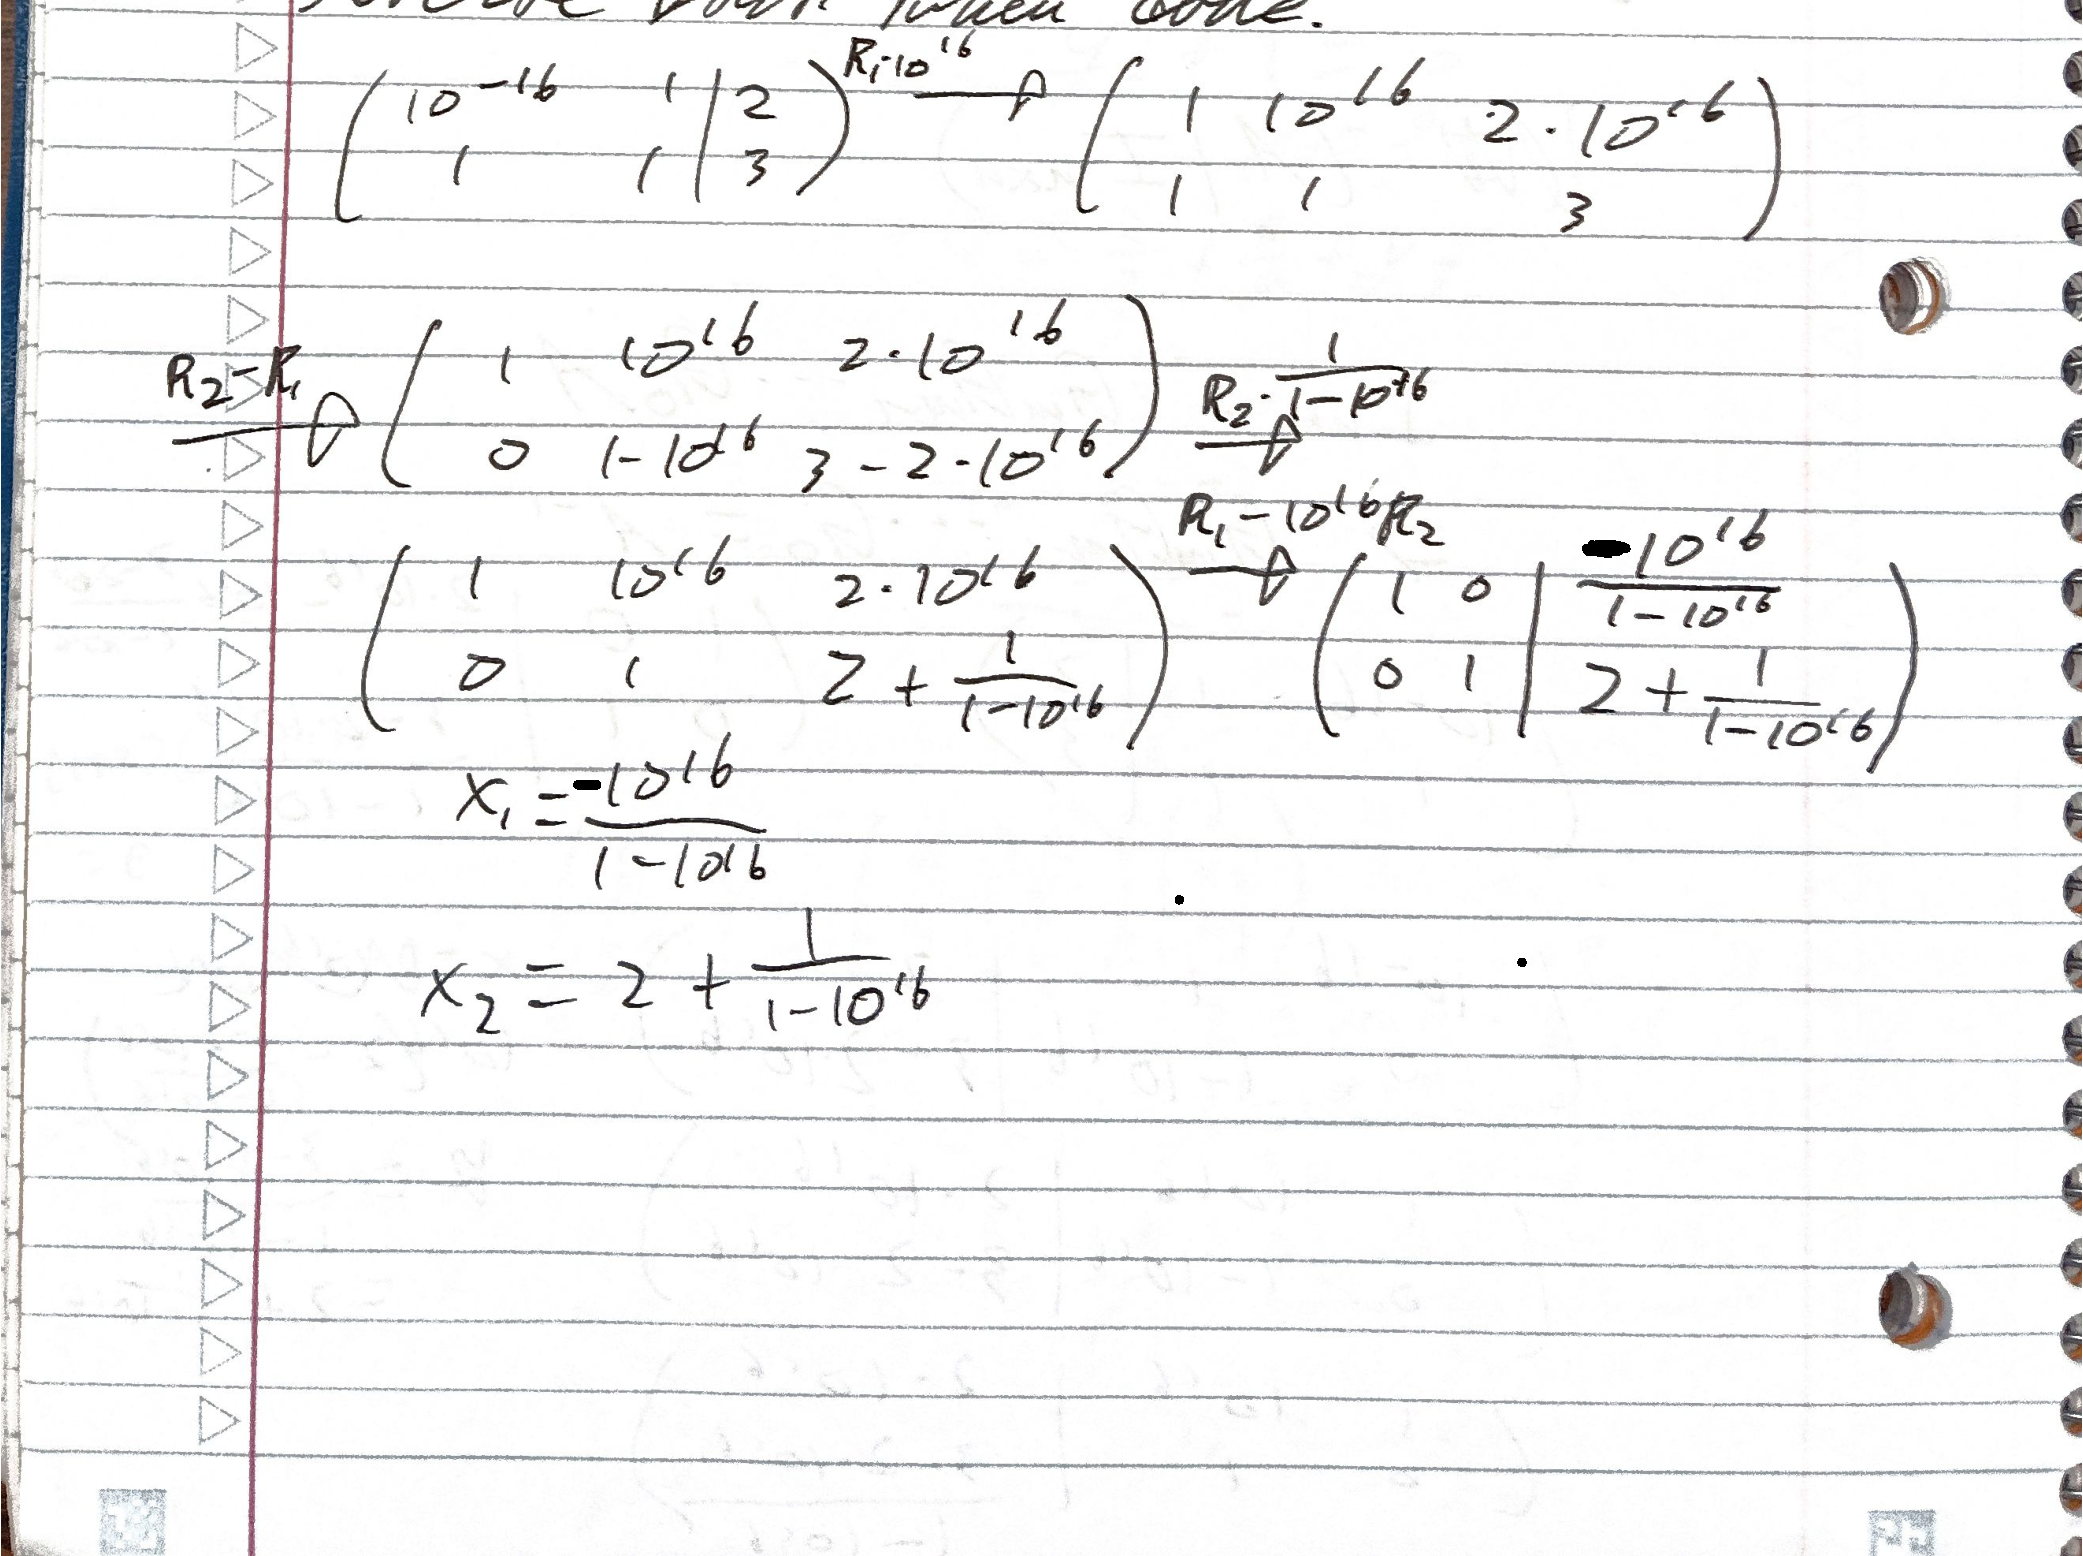
\includepdf{numAnalHWProb3ByHand.pdf}
			\item 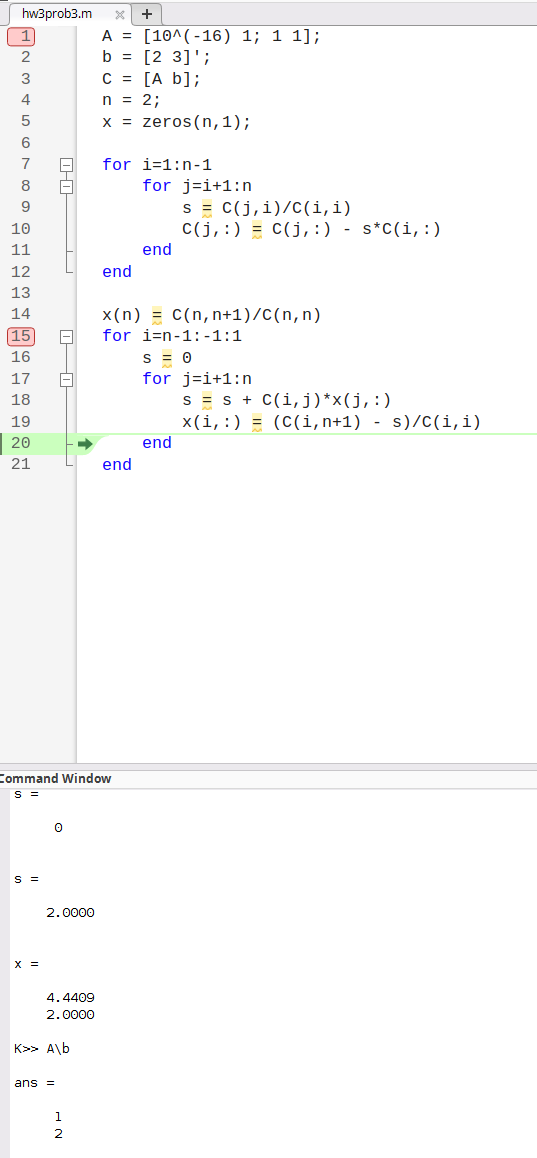
\includegraphics[scale=0.5]{numAnalHW4Prob3.png}
\end{enumerate}				
		\item{Question 4}
		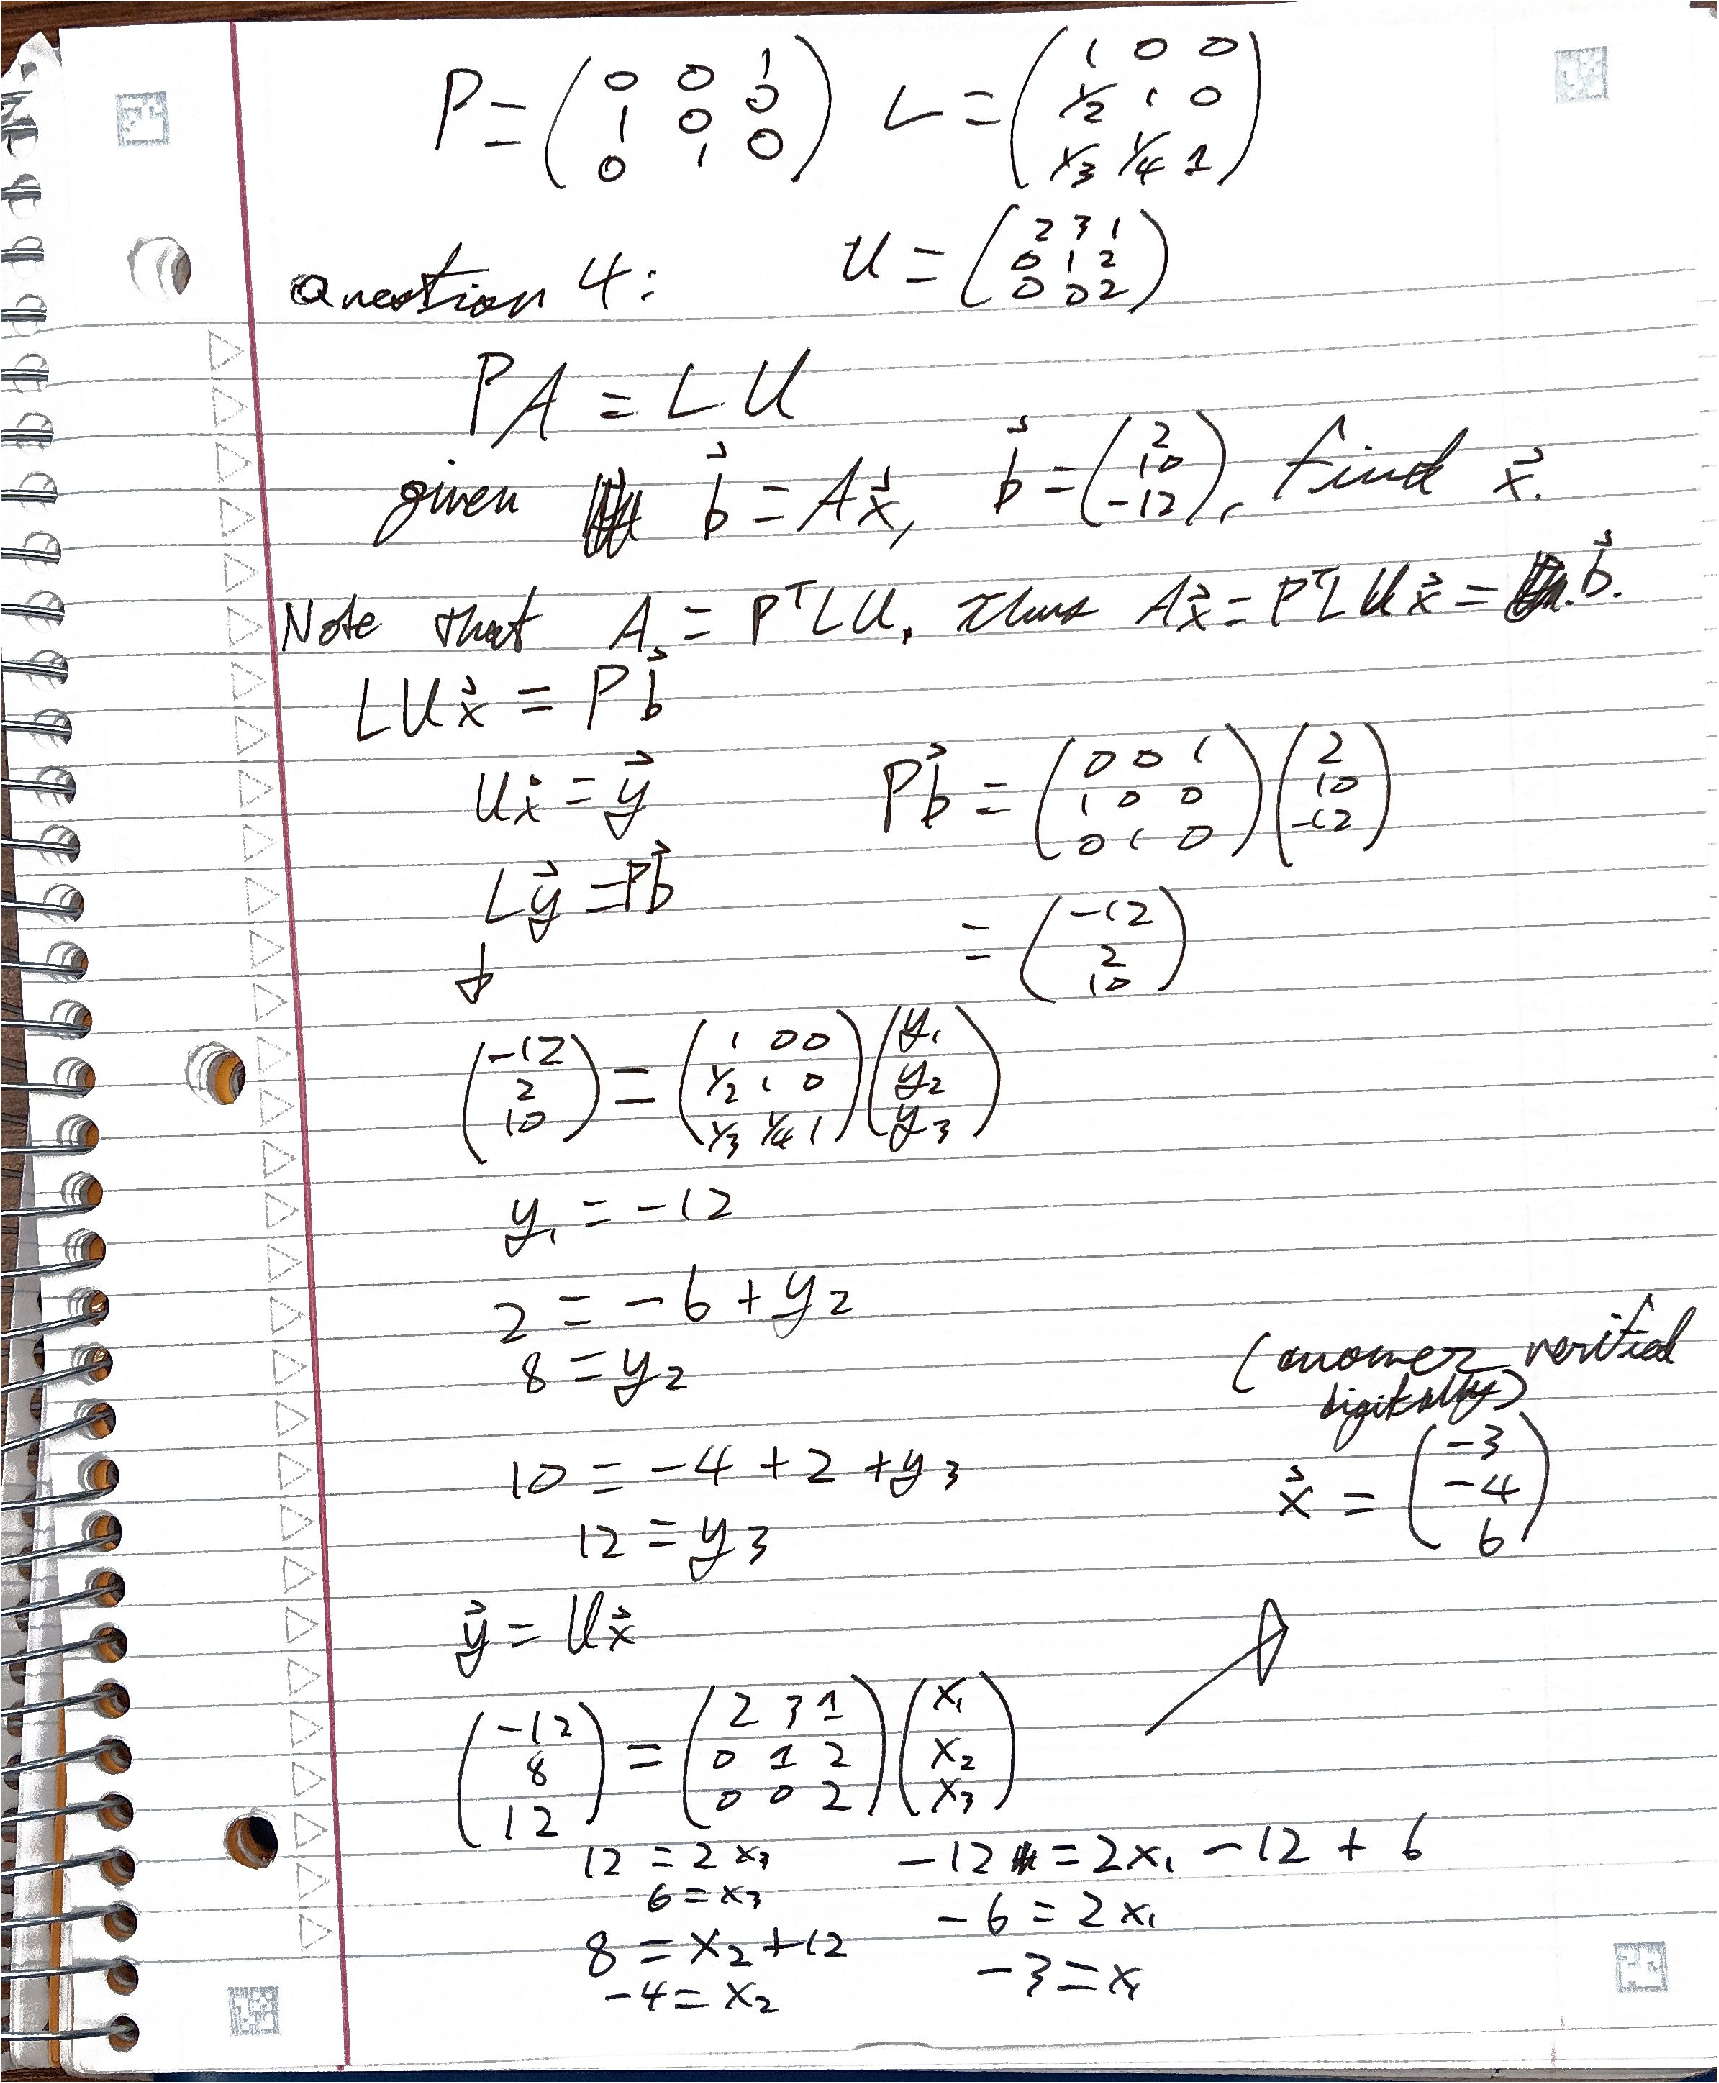
\includepdf{numanalHW3Prob4.pdf}
	\end{itemize}
\end{document}